\documentclass[12pt,a4paper]{beamer}
\usepackage[spanish,activeacute]{babel}
%\usepackage[latin1]{inputenc}
\usepackage[utf8]{inputenc}
%\usepackage[right=2cm,left=3cm]
\usepackage{mathrsfs}
\usepackage{mathtools}
\usepackage{amsthm}
\usepackage{graphicx}
\usepackage{amsfonts}
\usepackage{amsmath}
\usepackage{amssymb, setspace}

\usepackage{parskip}
\setlength{\parindent}{30pt}
\usepackage{ragged2e}

\theoremstyle{definition}
\newtheorem{thm}{Teorema}
\newtheorem{cor}[thm]{Corolario}
\newtheorem{lem}[thm]{Lema}
\newtheorem{prop}[thm]{Proposición}
\newtheorem{defn}[thm]{Definición}
\theoremstyle{remark}
\newtheorem{pru}[thm]{Prueba}
\newtheorem{rem}[thm]{Observación}

%\usepackage{a4wide}
\usepackage{color}
\usepackage{mathpazo} 
%\usepackage[scaled=.90]{helvet}
%\usepackage{cmtt}
%\renewcommand{\ttdefault}{cmtt}

\newcommand{\mathsym}[1]{{}}
\newcommand{\unicode}[1]{{}}

\usepackage{fancyvrb} 

\DefineVerbatimEnvironment{code}{Verbatim}
{fontsize=\normalsize,
 fontfamily=cmtt,
 fontshape=n,
 formatcom=\color{blue},
 frame=single}

\usetheme{Boadilla}
\usecolortheme{whale}
\useoutertheme{sidebar}
\useinnertheme{circles}

\AtBeginSection{
    \begin{frame}[c,noframenumbering]
        \tableofcontents[currentsection]
    \end{frame}
}

\title[Aproximación algebraica al problema SAT]{Una aproximación algebraica al problema SAT y su implementación funcional}
\author{Daniel Rodríguez Chavarría}
\institute[US]{Tutor: Joaquín Borrego Díaz \\ Cotutor: José Antonio Alonso Jiménez \\
\vspace{0.5cm} 
Departamento de Ciencias de la Computación e Inteligencia Artificial \\ Universidad de Sevilla}
\date{ 11 de Diciembre de 2017}

\setbeamertemplate{navigation symbols}{}
\begin{document}
\frame{\titlepage}

\begin{frame}
\tableofcontents
\end{frame}

\section{El Problema SAT}
\begin{frame}
\frametitle{El Problema SAT}
\framesubtitle{Satisfacibilidad de una fórmula}
En el marco de la lógica proposicional y asumiendo que se tiene un conocimiento básico de la misma,
\vspace{0.5cm}
\begin{defn}
Una fórmula se dice \alert{satisfacible} si existe al menos una valoración o
interpretación de la misma que sea modelo de ella.
\end{defn}
\end{frame}

\begin{frame}
\frametitle{El Problema SAT}
\framesubtitle{Enunciado}
\begin{center}
\huge{Sea $F$ una fórmula proposicional,}\\
\vspace{0.5cm}
\pause
\huge{¿Es satisfacible?}
\end{center}
\end{frame}

\begin{frame}
\frametitle{El Problema SAT}
\begin{itemize}
\item[•] Es un problema $NP$ completo ($NP + NP$-duro).
\item[•] Pieza clave en el problema $P$ versus $NP$, uno de los problemas del milenio.
\item[•] Debido a su gran importancia, tanto teórica como práctica, se celebra desde 2002 la \textit{SAT Competition}.
\end{itemize}
\end{frame}



\section{Método de refutación mediante omisión de variables}

\begin{frame}
\frametitle{\normalsize{Método de refutación mediante omisión de variables}}
\framesubtitle{Consideraciones del método}
Se aplicará el método a un conjunto de fórmulas (o base de conocimiento) en lugar de a una única fórmula.\\
\vspace{0.5cm}
Se resolverá determinando si el conjunto de fórmulas es inconsistente ya que una fórmula (o conjunto de fórmulas) es satisfacible si y sólo si no es inconsistente.
\end{frame}

\begin{frame}
\frametitle{\normalsize{Método de refutación mediante omisión de variables}}
\framesubtitle{Retracción conservativa}
\noindent Sean $K$ y $K'$ bases de conocimiento: 
\begin{defn}	
Se dice que $K'$ es \alert{retracción} de $K$ si $\mathcal{L}(K') \subseteq \mathcal{L}(K)$ y
 $$\forall F \in Form (\mathcal{L} (K')) \;\; [K' \vDash F \Rightarrow K \vDash
 F]$$
 Además, se dice que es \alert{conservativa} si también cumple:
 $$\forall F \in Form (\mathcal{L} (K')) \;\; [K \vDash F \Rightarrow K' \vDash
 F]$$
 \end{defn}
\end{frame}

\begin{frame}
\frametitle{\normalsize{Método de refutación mediante omisión de variables}}
\framesubtitle{Operador de omisión}
\begin{defn}
El operador $\delta :Form(\mathcal{L}) \times Form(\mathcal{L}) \rightarrow Form(\mathcal{L} \setminus \{ p \})$  es:

\begin{enumerate}
\item \alert{Correcto} si $\{F,G\} \vDash \delta (F,G)$.
\item Un \alert{operador de omisión} para la variable $p \in \mathcal{L}$ si 
$\{ \delta (F,G) \}$ es una retracción conservativa de la base de conocimiento $\{ F,G \}$ al lenguaje $\mathcal{L} \setminus \{ p \}$.
\end{enumerate} 
\end{defn}


\end{frame}

\begin{frame}
\frametitle{\normalsize{Método de refutación mediante omisión de variables}}
\framesubtitle{Lema de elevación}
\begin{lem}[de elevación]
 Sean $v :\mathcal{L} \setminus \{p\} \rightarrow \{ 0,1 \}$ una valoración o interpretación, $F, G \in Form(\mathcal{L})$ fórmulas y $\delta$ un operador de omisión de la variable $p$. Las siguientes condiciones son equivalentes:
\begin{enumerate}
\item $v \vDash \delta (F,G)$
\item Existe una valoración $\hat{v} : \mathcal{L} \rightarrow \{ 0,1 \}$ tal que $\hat{v} \vDash F \wedge G$ y $\hat{v} \upharpoonright_{\mathcal{L} \setminus \{ p \}} = v $
\end{enumerate}
\end{lem}
\end{frame}

\begin{frame}
\frametitle{\normalsize{Método de refutación mediante omisión de variables}}
\framesubtitle{Lema de elevación}
\begin{center}
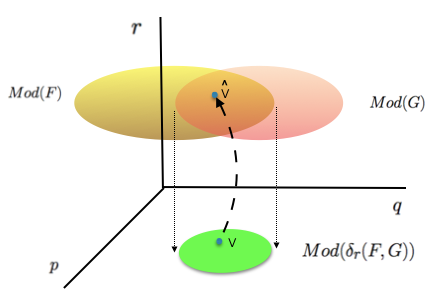
\includegraphics[scale=0.6]{imagenes/indemod.png}
\end{center}
\end{frame}

\begin{frame}
\frametitle{\normalsize{Método de refutación mediante omisión de variables}}
\framesubtitle{Extensión de $\delta$ y saturación}
\begin{defn}
Sean $\delta_p$ un operador de omisión de la variable $p$ y $K$ una base de conocimiento. Se define $\delta_p [\cdot ]$ como $\delta_p [K] := \{ \delta_p (F,G) : F,G \in K \}$.
\end{defn}
\begin{defn}
Suponiendo que se tiene un operador de omisión $\delta_p$ para cada $p\in \mathcal{L}$. Se llamará \alert{saturación} de la base de conocimiento $K$ al proceso de aplicar los operadores $\delta_p [\cdot ]$ (en algún orden) respecto a todas las variables proposicionales de $\mathcal{L}(K)$, denotando al resultado como $sat_{\delta}(K)$ (el cual será, por tanto, un subconjunto de $\{ \top , \bot \}$).
\end{defn}
\end{frame}

\begin{frame}
\frametitle{\normalsize{Método de refutación mediante omisión de variables}}
\framesubtitle{$\vdash_{\delta}$-refutación}
\begin{defn}
Sea $K$ una base de conocimiento, $F\in Form(\mathcal{L})$ y $\{ \delta_p : p \in \mathcal{L}(K) \}$ una familia de operadores de omisión.
\begin{itemize}
\item[•]Una  $\vdash_{\delta}$-prueba en $K$ es una secuencia de fórmulas $F_1, \dots ,F_n$ tal que para todo $i \leq n$, $F_i \in K$ ó existen $F_j , F_k (j,k < i)$ tal que $F_i = \delta_p (F_j , F_k)$ para algún $p \in \mathcal{L}$.
\item[•] $K \vdash_{\delta} F$ si existe una $\vdash_{\delta}$-prueba en $K$, $F_1, \dots ,F_n$, con $F_n = F$.
\item[•] Una $\vdash_{\delta}$-refutación es una $\vdash_{\delta}$-prueba de $\bot$.
\end{itemize}
\end{defn}
\end{frame}

\begin{frame}
\frametitle{\normalsize{Método de refutación mediante omisión de variables}}
\framesubtitle{Corrección del método}
\begin{thm}
Sea $\{ \delta_p : p \in \mathcal{L} \}$ una familia de operadores de omisión (correctos). Entonces $\vdash_{\delta}$ es refutacionalmente completo; es decir, $K$ es inconsistente si y sólo si $K \vdash_{\delta} \bot$.
\end{thm}
\noindent \textbf{Prueba:} La idea es saturar la base de conocimiento.
\begin{center}
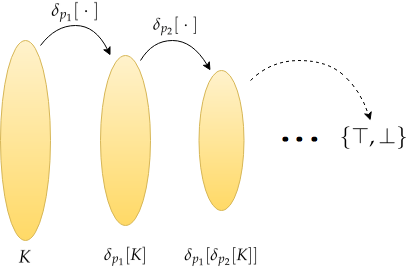
\includegraphics[scale=0.35]{imagenes/comple.png}
\end{center}
\end{frame}

\begin{frame}
\frametitle{\normalsize{Método de refutación mediante omisión de variables}}
\framesubtitle{Corrección del método}
Si $sat_{\delta} (K) = \{ \top \}$, entonces, aplicando repetidas veces el lema de elevación, se puede extender la valoración vacía (la cual es modelo de $\{ \top \}$) a un modelo de $K$.\\

Si $\bot \in sat_{\delta} (K)$ entonces $K$ es inconsistente, porque $K \vDash sat_{\delta} (K)$ al ser correctos los operadores. \hfill $\square$
\end{frame}

\begin{frame}
\begin{center}
\Huge{Ya tenemos el método, pero...}
\pause
\Huge{¿Quién es $\delta$?}
\end{center}
\end{frame}

\begin{frame}
\frametitle{Regla de independencia}
\begin{defn}
La regla de independencia se define como:
$$\partial_p(F_1,F_2) = \Theta (\partial_{x_p} (\pi (F_1),\pi (F_2)))$$
\end{defn}
\end{frame}

\section{Interpretación algebraica de la lógica}
\begin{frame}
\frametitle{Interpretación algebraica de la lógica}
%\framesubtitle{Esquema}
\vspace{1cm}
\begin{center}
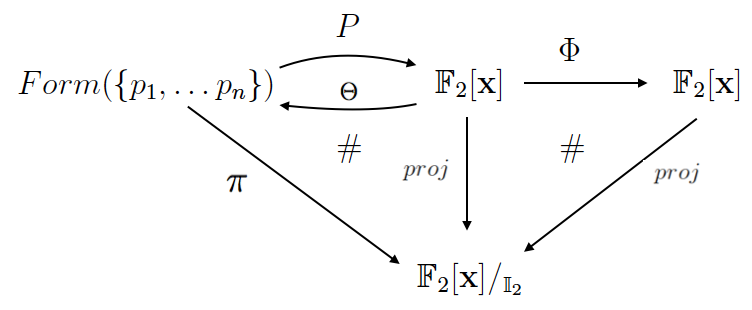
\includegraphics[scale=0.35]{imagenes/conmu.png}
\end{center}
\end{frame}

\begin{frame}
\frametitle{Interpretación algebraica de la lógica}
\framesubtitle{De fórmulas a polinomios}
\begin{defn}
Se define la función $P: Form\{\mathcal{L}\} \rightarrow \mathbb{F}_2[\textbf{x}]$ por:
\begin{itemize}
\item[•] $P(\perp)=0$, $P(p_i)=x_i$, $P(\neg F)=1+P(F)$
\item[•] $P(F_1 \wedge F_2) = P(F_1) \cdot P(F_2)$
\item[•] $P(F_1 \vee F_2) = P(F_1) + P(F_2) + P(F_1) \cdot P(F_2)$
\item[•] $P(F_1 \rightarrow F_2) = 1 + P(F_1) + P(F_1) \cdot P(F_2)$
\item[•] $P(F_1 \leftrightarrow F_2) = 1 + P(F_1) + P(F_2)$
\end{itemize}
\end{defn}
Por ejemplo,
$$P(p \wedge (q \vee r)) = P(p) \cdot P(q \vee r) = $$
$$= x_p \cdot (x_q+x_r+x_q \cdot x_r) = x_px_qx_r+x_px_q+x_px_r$$
\end{frame}

\begin{frame}
\frametitle{Interpretación algebraica de la lógica}
\framesubtitle{De polinomios a fórmulas}
\begin{defn}
Se define la función $\Theta: \mathbb{F}_2[\textbf{x}] \rightarrow Form\{\mathcal{L}\}$ por:
\begin{itemize}
\item[•] $\Theta (0) = \perp$
\item[•] $\Theta (1) = \top$
\item[•] $\Theta (x_i) = p_i$
\item[•] $\Theta (a+b) = \neg(\Theta(a) \leftrightarrow \Theta(b))$
\item[•] $\Theta (a \cdot b) = \Theta(a) \wedge \Theta(b)$
\end{itemize}
\end{defn}
Notar que $\Theta$ no es la inversa de $P$.
\end{frame}

\begin{frame}
\frametitle{Interpretación algebraica de la lógica}
\vspace{1cm}
\begin{center}
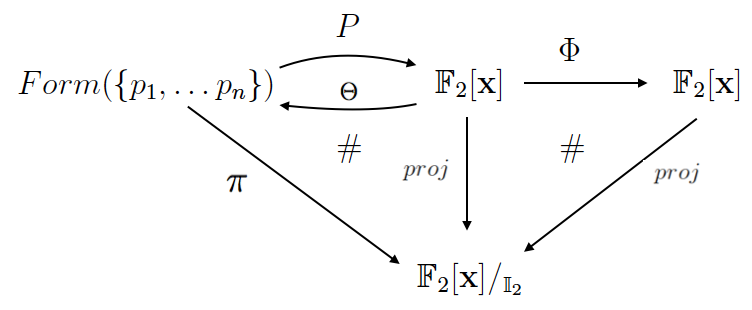
\includegraphics[scale=0.35]{imagenes/conmu.png}
\end{center}
\end{frame}

\begin{frame}
\frametitle{Interpretación algebraica de la lógica}
\framesubtitle{Proyección polinomial}
\begin{defn}
Se define la función $\Phi$ por:
 $$\Phi:\mathbb{F}_2[\textbf{x}] \rightarrow \mathbb{F}_2[\textbf{x}]$$
 $$\Phi (\sum\limits_{\alpha \in I} \textbf{x}^{\alpha} ) := \sum\limits_{\alpha
 \in I} \textbf{ x}^{sg(\alpha)} $$

 \noindent siendo $sg(\alpha) := (\delta_1 ,\dots,\delta_n)$ donde $\delta_i$ es 0 si
 $\alpha_i = 0$ y 1 en cualquier otro caso.
 \end{defn}
\end{frame}

\begin{frame}
\frametitle{Interpretación algebraica de la lógica}
\framesubtitle{Transformación polinomial}
\noindent Finalmente,\\
\vspace{0.5cm}
\begin{defn}
La función que define la transformación es:
$$\pi = \Phi \circ P$$
\end{defn}
\end{frame}

\section{Regla de independencia}
\begin{frame}
\frametitle{Regla de independencia}
\framesubtitle{Recapitulando}
\begin{defn}
La regla de independencia se define como:
$$\partial_p(F_1,F_2) = \Theta (\partial_{x_p} (\pi (F_1),\pi (F_2)))$$
\end{defn}
\end{frame}

\begin{frame}
\frametitle{Regla de independencia}
\framesubtitle{Polinomios}
\begin{defn}
Dados $a_1,a_2 \in \mathbb{F}_2 [\textbf{x}]$ y $x$ una variable indeterminada, la \alert{regla de independencia} (o regla $\partial$) sobre fórmulas polinomiales se define como sigue: \\
\vspace{0.2cm}
\begin{table}[h]
\centering
\begin{tabular}{c}
$a_1$, $a_2$ \\
\hline $\partial_x (a_1,a_2)$
\end{tabular}
\end{table}

\vspace{0.2cm}
\noindent donde:\\
$$\partial_x (a_1, a_2) = 1 + \Phi [(1+a_1 \cdot a_2) \cdot  $$$$ (1+a_1 \cdot \frac{\partial}{\partial x} a_2 + a_2 \cdot \frac{\partial}{\partial x} a_1 + \frac{\partial}{\partial x} a_1 \cdot \frac{\partial}{\partial x} a_2)]$$

\end{defn}
\end{frame}

\begin{frame}
\frametitle{Regla de independencia}
En el trabajo se prueba que esta regla es un operador correcto y de omisión; por tanto, es fácil ver que dada una base de conocimiento, $K$ :\\
\vspace{0.5cm}

\begin{cor}
$K$ es inconsistente si y sólo si $K\vdash_{\partial} \bot$.
\end{cor}
\end{frame}

\section{SAT$\_$Solver}
\begin{frame}
\frametitle{SAT$\_$Solver}
\framesubtitle{Tecnologías}
\begin{enumerate}
\item Lenguaje funcional Haskell.
\item Stack.
\item Haskell Literario.
\item Librerías como \texttt{HaskellForMaths}, \texttt{doctest} o \texttt{quickCheck}.
\item Git y GitHub.
\end{enumerate}
\end{frame}

\begin{frame}
\frametitle{SAT$\_$Solver}
\framesubtitle{Estructura de la herramienta}
El proyecto está formado por 9 módulos, aunque la herramienta se divide principalmente en dos etapas secuenciales:
\begin{enumerate}
\item Preprocesado del fichero de entrada en formato \texttt{DIMACS}
\item Saturación del conjunto de polinomios y decisión.
\end{enumerate}
\end{frame}

\begin{frame}
\frametitle{SAT$\_$Solver}
\framesubtitle{Demostración}
\begin{center}
\Large{Ejemplo de uso desde consola}\\
\vspace{0.5cm}
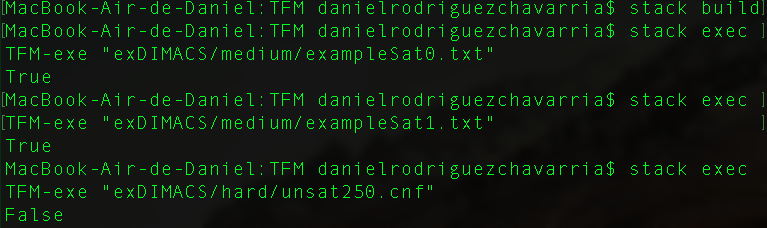
\includegraphics[scale=0.37]{imagenes/example.png}
\end{center}
\end{frame}

\section{Conclusiones y trabajos futuros}
\begin{frame}
\frametitle{Conclusiones y trabajos futuros}
Destacan tres líneas de investigación:
\begin{itemize}
\item[•] Mejorar la eficiencia de la implementación
\item[•] Extender el modelo a lógicas multi-valuadas
\item[•] Dar de explícitamente el algoritmo formal, estudiando su complejidad computacional teórica.
\end{itemize}
\end{frame}

\begin{frame}
\frametitle{Conclusiones y trabajos futuros}
Desarrollando la primera:
\begin{enumerate}
\item Implementar una librería de polinomios específica.
\item Tratar de encontrar alguna propiedad que permita reducir el número de polinomios de una base de conocimiento, ya que, el principal problema detectado es de espacio computacional.
\item Profundizar en el estudio de heurísticas a fin de encontrar una que se adecúe mejor al problema, por ejemplo, ayundándonos del aprendizaje automático.
\end{enumerate}
\end{frame}
\begin{frame}
\frametitle{Conclusiones y trabajos futuros}
\begin{enumerate}
\setcounter{enumi}{3}
\item Tratar de incluir la paralelización de procesos, por ejemplo, mediante el cálculo de la regla de independencia de conjuntos con variables disjuntas. 
\item Se podría combinar este método con otros más eficientes a la hora de responder afirmativamente al problema de satisfacibilidad, por ejemplo, con métodos de fuerza bruta o el DPLL.
\end{enumerate}
\end{frame}

\begin{frame}[allowframebreaks]
  \frametitle{Bibliografía}
  \nocite{formulasYpolinomios}\nocite{original}
\bibliographystyle{abbrv}
\bibliography{TFM}

\end{frame}

\begin{frame}
\centering
	\Huge{Gracias por la atención} \\
	\pause
	\vspace{0.5cm}
	\Huge{¿Preguntas?}\\
	\pause
	\vspace{0.5cm}
	\Huge{Demostración}

\end{frame}

\end{document}
